\chapter{Architektur}

\section{Der Hub}
\sectionauthor{\leonard}

Der \emph{Spielehub} ist der zentrale Zugangspunkt und auch das Erste was der 
Nutzer sieht, wenn er die App startet. Dieser ist in 3 Teile aufgespalten und besitzt 
eine seitliche Navigationsleiste (\emph{Navigation-Drawer}). Jedes Teil ist dabei
ein \code{Fragment}. Der \code{Hub} besteht aus dem \emph{Spielehub}, welcher 
die Spielstände als Liste hält, den \emph{Kartenspielen} und den \emph{Brettspielen}.


\subsection{Naviagtion Drawer}

Als Menu verwenden wir einen \emph{Navigation-Drawer}, welcher nur im \code{Hub} 
zur Verfügung steht und wie folgend aufgebaut ist. 

\section{Die Spielstände}
\sectionauthor{\leonard}

Da man Spiele nicht immer in einem Zug durchspielt und man zwischendurch Pause
macht, ist es sinvoll das Speichern und Laden der Spiele zu ermöglichen. Für
diese Funktion sind die Klassen \code{SavegameStorage}, \code{Savegame} und
\code{SavegameAdapter} zuständig.

\subsection{Klassen}

\code{Savegame} ist das Spielstand-Objekt, welches alle Daten speichert, die
nötig sind um ein Spiel fortsetzen zu können. Jedes \code{Savegame} ist dabei
einzigartig.

\code{SavegameStorage} kümmert sich um das Speichern und Laden der
\code{Savegame} Objekte. Diese werden als Liste serialisiert und auf dem Gerät
gespeichert.

\code{SavegameAdapter} erstellt aus den gepeicherten \code{Savegame} Objekten,
für jeden Spielstand eine Karte, welche im Startbildschirm in einer Liste
angezeigt wird. Die Klasse ist etwas komplizierter aufgebaut als die anderen.
Sie besitzt innere Klassen, Vererbungen und eine Interface Implementierung.

\begin{figure}[h]
	\centering
	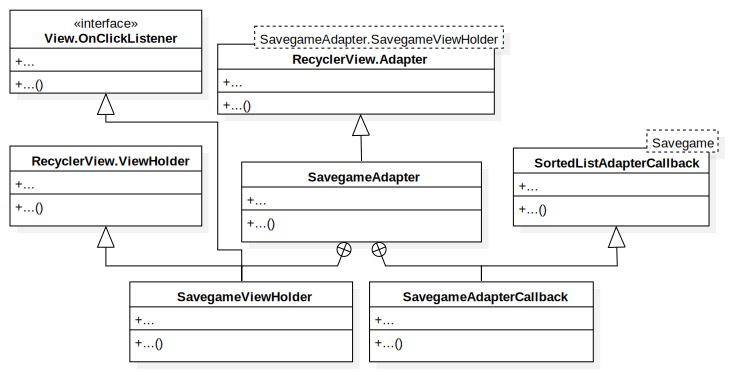
\includegraphics[width=1.0\textwidth]{resources/savegamestorage/SavegameAdapter}
	\caption{Spielstand SavegameAdapter}
\end{figure}

\subsection{Aufbau}

Wenn ein Spiel gespeichert oder geladen werden soll, so geschieht dies durch
einen Aufruf der Instanz \code{SavegameStorage}. Um hier nicht ständig neuen
Code schreiben zu müssen, haben wir diese Aufgabe in die Klasse
\code{GameActivity} gelegt. Da jedes Spiel von \code{GameActivity} erben sollte,
müssen dadurch zwei abstrakte Methoden implementiert werden, welche genau
hierfür zuständig sind. Die Methode zum Laden heißt \code{onLoadGame} und die
Methode zum Speichern \code{onSaveGame}. Diese Methoden arbeiten lediglich mit
einem \textbf{Bundle}, welches die nötigen Informationen beinhaltet. Beim
Speichern sollten also alle wichtigen Informationen hinzugefügt werden, damit
man dann beim Laden Zugriff auf jene hat.

\begin{figure}[h]
	\centering
	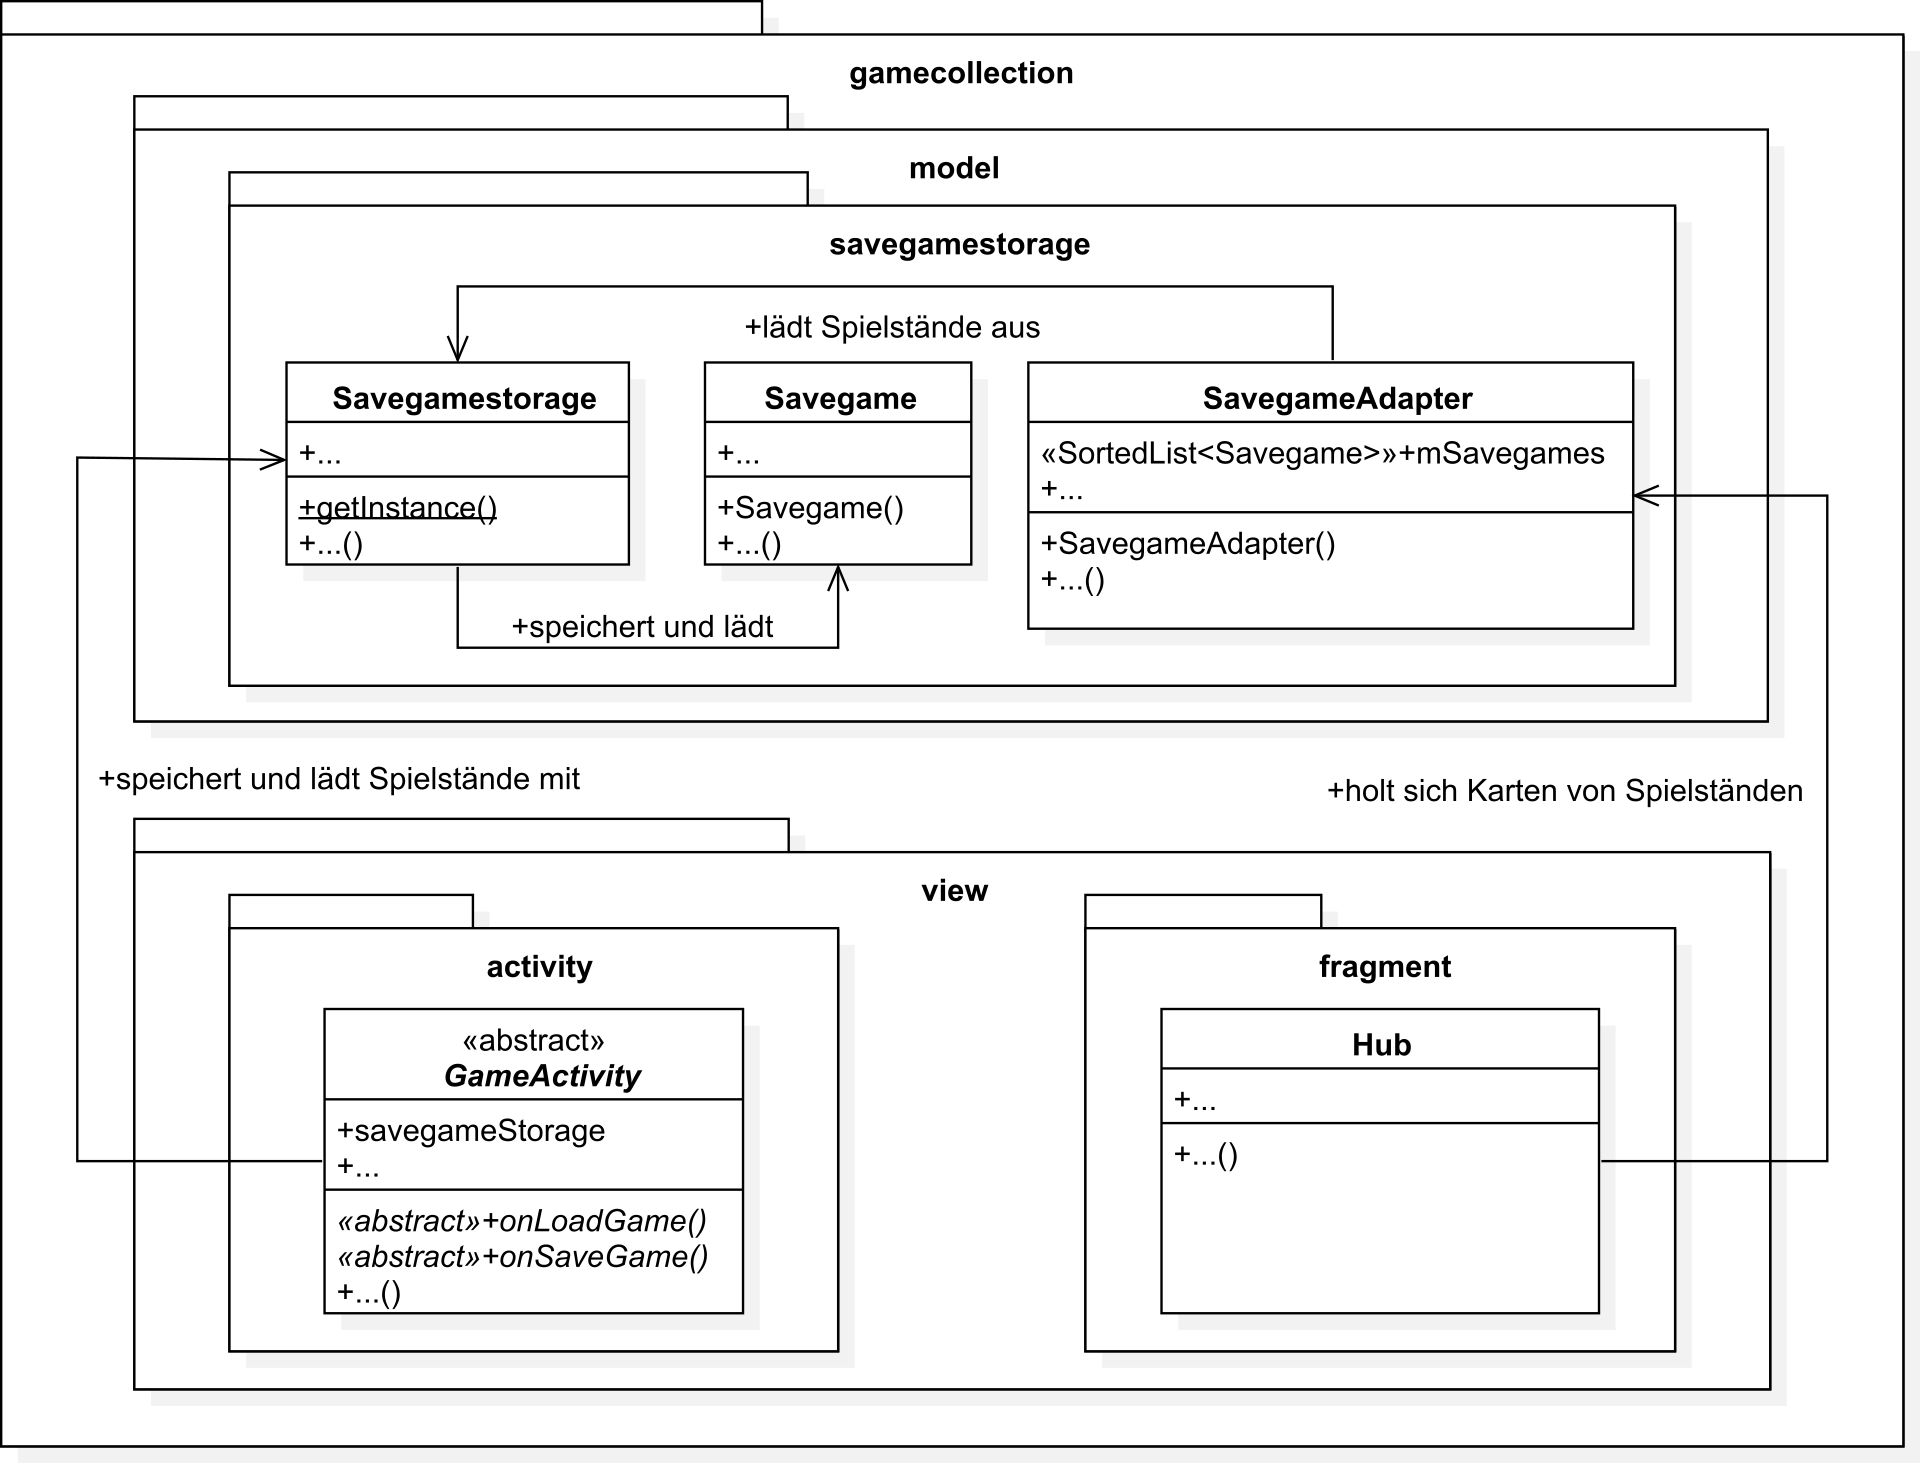
\includegraphics[width=1.0\textwidth]{resources/savegamestorage/Savegamestorage}
	\caption{Spielstand Architektur}
\end{figure}